\documentclass[10pt]{article}
\include{the_workbook_preamble}
%\usepackage[breaklinks=true]{hyperref}
%\usepackage[margin=0.75in]{geometry}
%
%\usepackage{graphicx}
%\usepackage{color}
%
%\definecolor{pblue}{rgb}{0.13,0.13,1}
%\definecolor{pgreen}{rgb}{0,0.5,0}
%\definecolor{pred}{rgb}{0.9,0,0}
%\definecolor{pgrey}{rgb}{0.46,0.45,0.48}
%
%\usepackage{listings}
%\lstset{language=Java,
%  showspaces=false,
%  showtabs=false,
%  tabsize=2,
%  breaklines=true,
%  showstringspaces=false,
%  breakatwhitespace=true,
%  commentstyle=\color{pgreen},
%  keywordstyle=\color{pblue},
%  stringstyle=\color{pred},
%  basicstyle=\ttfamily,
%  frame=single,
%  moredelim=[il][\textcolor{pgrey}]{$$},
%  moredelim=[is][\textcolor{pgrey}]{\%\%}{\%\%}
%}

\title{Java Collections Part 1}
\author{
	Melvyn Ian Drag
}
\date{\today}


\begin{document}
\maketitle

\begin{abstract}
$java.util$ provides many containers. These containers are widely used in Java programming and are implementations of the great data structures you hear about in data structures \& algorithms classes. In today's lecture we'll have a look at a few of them and consider when we would want to use them.

We will also review how to convert between numeric types. This is a basic CS
topic that you might have forgotten, but need to understand for our final
project.
\end{abstract}

\section{Start with the math stuff}
It is important that you know how to convert numbers between base 2 ( binary),
base 10 ( decimal ) and base 16 (hexadecimal, usually people just say "hex" )

Pretty much we just think of every digit as powers of the base.

So in base 10:
10*0, 10**1,  10**2, etc..

in base 2:
2**0, 2**1, 2**3

and in base 16:
16**0, 16**1, 16**2


Example 1:
convert 6574 base10  to base 2, then convert back to base 10

Whats the largest power of 2 that goes in?
1,2,4,8,16,32,64,128,256,512,1024,2048, 4096=2**12, 8192 = 2**13 so 2**12 is the
biggest one. 2**12 with be the 13th bit ( dont forget the 0 bit, indexing starts
at 0,not 1 )
Then the remainder is 6574 - 4096 = 2478
Then we can take one 2**11 from that 2478 - 2048 = 430
The n we can take one 2**8 from that 430 - 256 = 174
And we can take one 2**7 from there 174 - 128 = 46
Then we can take one 2**5 from there 46 - 32 = 14
Then take one 2**3 from there 14 - 8 = 6
Then take a 2*2 from there 6 - 4 = 2
Then we are left with a single 2**1
So the binary must be 
1100110101110

in other words:
1 2**12
1 2**11
0 2**10
0 2**9
1 2**8
1 2**7
0 2**6
1 2**5
0 2**4
1 2**3
1 2**2
1 2**1
0 2**0

And that is how decimal to binary conversion works.

To go from binary to decimal, just add the powers of 2. 
So this would be 
2**12 + 2**11 + 2**8 +...

Weve printed left to right the 13th down to the 0th bit.

Why do we care about Binary numbers?!?! What's the point of this?! 
In this class we will doing real computer science. We will be manipulating bits.
Sometimes you will want to manipulate bits in your hardware. You'll want to know
what the 1s and 0s are in your computer for some reason. Binary numbers tell you
explicitly what numbers are in your computer. You know computers use
electricity? If there is a high voltage the computer interprets that as 1. If
ther eis a low voltage the computer takes that to be a zero. And with just that
your computer can do crazy stuff like send emails ,drive cars, solve math
problems. Sometimes youll need to get your hands dirty and look at the 1s and
0s.

NOTE! we havent talked about sign bits yet. Java numbers are all + or -. Well
need to look at the conversion from decimal to a signed binary number. We will
talk about taht later, it requires a little more thinking on your part so I just
want you to show me that you understand this first.

\subsection{Working with hex numbers.}

What is the point of hex numbers?! The point is hex numbers are awesome at
storing 8 bit  binary numbers in just 2 chatracters. And its super easy and
beautiful to go bac kand forth between hex and binary.

First lets look at decimal to hex.

its the same as decimal to binary .Except now we work with powers of 16 and not
2.

16**0 = 1
16**1 = 16
16**2 = 256
16**3 = 4096

So lets convert our old friend 6574 to hex.

There is 1 4096. Remainder is 6574 - 4096 = 2478
In there there are 9 16**2s. 256 * 9 = 2304. And 2478 - 2304 = 174
And there are 10 number 16**1s in there. 174 - 10*16 = 14.
And then there are 14 ones.
So the digits in our hex number would be 
1, 9, 10, 14 corresponding to 1 16**3, 9 16**2, 10 16**1 and 14 16**0.
By convention, for convenience, we write hex 10 as A, hex 14 as E.
So the number in hex is 19AE.

\subsection{Going the other way, hex to decimal}
This is just as with binary. Its easier to do hex to decimal than decimal to
hex. Just multiply like this: 1*16**3 + 9 * 16**2 + 10*16**1 + 14 * 16**0

\subsection{And now the beautfiful thing}
I hope you see the beauty in what were doing. If not yet, then this bit here
will knock your socks off.

[consider reviewing the three pillars of OOP really quick ]

Ok now that Im sure you know the pilars of oop let me show this other thing we
were talking about


take a binary number and make sure it has a multiple of 8 digits. 

Take tihs one 10011 this has only 5. Lets put some zeros on the left ot make it
8

00010011. 

thats better

To go to hex, first split it into two groups of four. Oh this is why its so
beautiful

0001    0011


Now turn each of the halves into decimal


1       3

And then turn the decimals into hex.

13

and thats how you write a byte in hex!!

Heres another one

11111100

convert to hex

easy

there are 8 bits already so good.

Then split in two

1111 1100


then each half to decimal

15   12


then each half to hex

FC


done!

By the way, you can write the hex numbers in caps or lowercase, but dont mix
that would be uncommon. FC and fc is good. fC or Fc woulc be unusual and probaly
jpeople would look at you weird.



Okay and now lets look at that number 6574 again. 

In binary we found it to be

1100110101110

Lets break it into 8 bit bytes

11001 10101110

pad on the left with 0s

00011001 10101110

Now break the bytes into groups of 4


0001 1001 1010 1110

and now convert each one to dcimal

1    9    10   14

and then to hex

19 AE


Which is exactly what we found earlier. 

There are other ways to do these conversions. If you know another way that's
great .Some are faster some are shorter. I think this method is straight forward
and algorithmic. As you practice it will become super easy to do. If you dont
practice it might be confusing.

I've given you a homework assignment to do this.


\section{Introduction}
A java collection is a container you can use to store a bunch of values. For example, in your program you may need to store a bunch of ages - in this case you would

\begin{lstlisting}[style=java]
...
int[] ageArray = {19, 25, 13, 41, 15};
...
\end{lstlisting} 

or you might create a class called 'Person' and when want to store a bunch of People. In this case you might

\begin{lstlisting}[style=java]
Person[] peopleArr = { new Person(), new Person(), ...};
\end{lstlisting}

in these two examples I am using arrays. While arrays are fine for simple collections of items, there are some distinct disadvantages of using arrays compared to using a more elegant container. There are some cases where using an array is extremely problematic. One major disadvantage is that the array size is fixed. Once you create an array of 5  elements , you cannot add a sixth person to the array.  

There are many Java Collections. For example, 

\begin{enumerate}
\item ArrayList
\item LinkedList
\item Vector
\item PriorityQueue
\item ArrayDeque
\item HashSet
\item LinkedHashSet
\item TreeSet
\item HashMap
\item TreeMap
\item LinkedHashMap
\item ConcurrentListSkipMap
\item WeakHashMap
\item Stack
\item etc.
\end{enumerate}

We are going to focus on just a few of them today. Namely, we will compare

\begin{enumerate}
\item ArrayList
\item LinkedList
\end{enumerate}


\section{The Collections Interface}
As we've discussed in this class, an interface is one way that Java does
inheritance. Interfaces provide a set of methods that the implementations must
implement. Here are the methods provided by the collections interface:

\begin{lstlisting}[style=java]
boolean add(E e)
boolean addAll(Collection<? extends E> c)
void clear()
boolean    contains(Object o)
boolean     containsAll(Collection<?> c)
boolean     equals(Object o)
int     hashCode()
boolean     isEmpty()
Iterator<E>     iterator()
default Stream<E>     parallelStream()
boolean     remove(Object o)
boolean     removeAll(Collection<?> c)
default boolean     removeIf(Predicate<? super E> filter)
boolean     retainAll(Collection<?> c)
int     size()
default Spliterator<E>     spliterator()
default Stream<E>     stream()
Object[]     toArray()
<T> T[]     toArray(T[] a)
\end{lstlisting}

reference:
\url{https://docs.oracle.com/javase/8/docs/api/java/util/Collection.html}

Have a look at the methods above and you will see that there are many useful
methods for working with a collection of things.

\section{Hands On Practice}
Now we will play with these collection methods.

There are a bunch so we'll go through them one at a time.
Here is a code listing for the practice iwth students. Feel free to include or
exclude print statements as time allows.

\lstinputlisting[style=java]{TestCollectionAPI.java}

\begin{figure}[h]
  \centering
    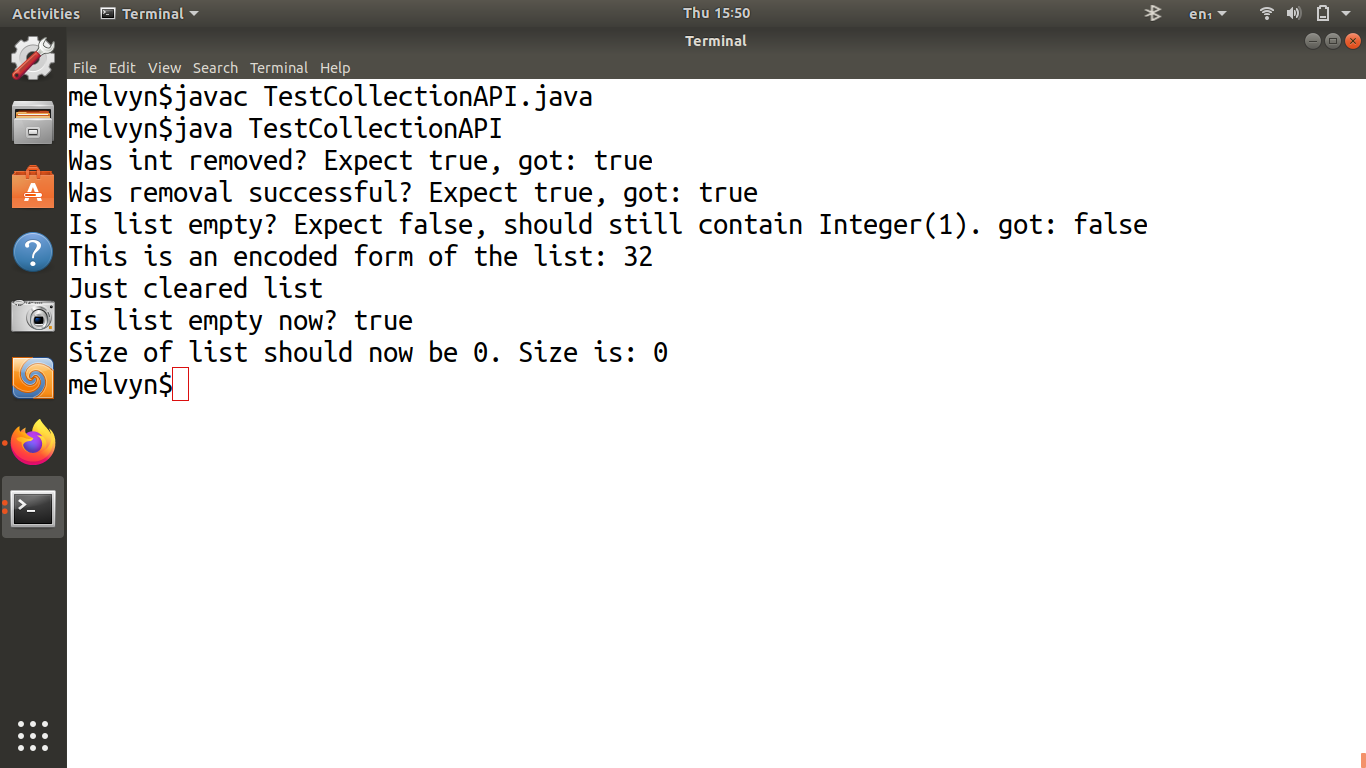
\includegraphics[width=0.5\textwidth]{outputOfCollectionsAPIExperiment.png}
  \caption{Illustration of a variety of classes which implement the Collection class.}
\end{figure}


\section{Implementations of Collection Interface and the Children of Those
Implementations}
Now we can have a look at the classes the implement this Interface.
We will look through the hierarchy all hte way down until we reach the
Collections we are interested today.

The takeaway I expect you to have from the next few minutes is some comfort with
reading technical documentation. When they asked me to teach this class 3 years
ago, I only knew a bit about Java that I had to learn for school and for work. I
was able to prepare a fairly decent lecture because I knew how to read the
documents! Everything about Java is there on the internet, you just need a few
minutes to sit and patiently read and digest what you've read.

Today we are talking about Lists in particular. Let me show you a couple of
things:
\url{https://docs.oracle.com/javase/8/docs/api/java/util/LinkedList.html}
There  is the official oracle documentation for the LinkedList class.
Look near the top and see that  Linked List is an object, an AbstractCollection,
an Abstract List, and AbstractSequentialList, and implements interfaces
Serializable, Cloneable,  Iterable, a Deque, a List and a Queue.
If you want the full story about what the Java implementation of  a LINked List
can do you can look through the documentation for each one of the base classes
and interfaces. We will do that later in the semester as an exercise. For now
we're just looking at the basic methods of the class.

\subsection{Iterating over a collection and doing stuff to it}
There are a few ways to iterate over a java collection. 

Sometimes you want to walk over the elements in a collection.

Heres how to do it with a forloop

\lstinputlisting[style=java]{ForLoopList.java}

Heres how to do it with an iterator

\lstinputlisting[style=java]{IteratorList.java}

And here is a way to iterate over a list and perform the same operation to every
element in this list. This is often referred to as a map operation:
\lstinputlisting[style=java]{StreamExample.java}


\section{What is a list?}
A list is an abstract idea - it's a bunch of objects in a row, like the arrays that we've seen so far. The list contains a bunch of items. You can delete items from it and add items to it. As I said before - big drawback of arrays is that the size of an array is fixed.

\lstinputlisting[style=java]{IntArrayCreator.java}

Note that all of the above arrays have four elements in them, and that cannot be changed! Sometimes that's what you want, sometimes thats not. Your call. If you want a variable number of elements in your container, use a List not an array.

\section{What is an ArrayList?}
\subsection{overview}
An ArrayList is a container like an array, but the size isn't fixed. You can put some elements of a specified type in them. See this example to create ArrayLists of different types:

\lstinputlisting[style=java]{ArrayListDemo.java}

WARNING! This code won't work:
\begin{lstlisting}[style=java]
...
ArrayList<int> intArrayList = new ArrayList<int>();
...
\end{lstlisting}

because you can't put primitive types in an ArrayList - only reference types ( i.e. everything except primitives )
You can't put any of these in an ArrayList

\begin{itemize}
\item byte
\item float
\item int
\item double
\end{itemize}

but the ``Byte", ``Float", ``Int" and ``Double" types are okay, because these aren't primitives, they are classes.


\section{Exercise: Create 5 different ArrayLists, each holding a different type.}

Allow 10 minutes to ensure that everyone can use the arraylists successfully.


\section{What is a LinkedList?}
To be perfectly honest, I've not yet researched how linked lists are implemented in Java, but I have studied algorithms and I've see how they are implemented in other languages. I'll give you a bit of information now and then we'll do some experiments to see if Java aligns with our expectations.


\textit{Read the wikipedia article on linked lists}

I will improvise this section about a linked list. If you don't understand the concept after our discussion in class, you can look on youtube. Sometimes hearing different people say the same things makes those things easier to understand.

\section{The Collections Interface}
Here is a good picture I found to explain the collections interface:

\begin{figure}[h]
  \centering
    \includegraphics[width=0.5\textwidth]{java-collection-hierarchy.png}
  \caption{Illustration of a variety of classes which implement the Collection class.}
\end{figure}


What are some methods that the  collections interface supplies?

\subsection{Exercise}
I could have written a long lesson on this, but I think it's better that we just find out together. I'm not sure what the collection interface supplies - I could spend an hour now researching and implementing some code, but why don't we do it together?

\subsection{Reference}

\url{https://www.javatpoint.com/collections-in-java}

\section{Initializing a List\textless T\textgreater with an ArrayList\textless T\textgreater or LinkedList\textless T\textgreater}
Weird thing that Java programmers do. Java programmers use this pattern to achieve a bunch of complex things that you won't learn about in this class. Grab a good book and learn to write a Java Web App or Android App and you will see this pattern used in certain ways to achieve particular ends.

\begin{lstlisting}[style=java]
List<String> l = new ArrayList<String>(){"Hello", "World"};
\end{lstlisting}

\section{Timing Comparison}
In this section we'll measure how long different datastructures take to perform different tasks. The reason different data structures exist is that they have different strengths and weaknesses, and programmers might need a datastructure that performs well in a certain situation. This talk is somewhat abstract if you haven't taken  a data structures and algorithms class. There you learn things like ``Computational Complexity" and ``Big O" notation. We're only going to focus now on the simplest of examples to give you a taste of whats to come ( for those who haven't yet studied data structures). For those who already know about datastructures, I'm hoping you're still interested in discussing them.

\subsection{How To Time Code}
There are many ways to measure time with Java. I'll just show you one. Java knows how many milliseconds have passed since the \textbf{Epoch}. When is the Epoch? Why is it important I can't remember, but it is a commonly used "t0" in computer science, especially on unix systems. 

Do the add and remove operations. Discuss the complexity of those operations, and then work it out in class.

\subsection{Timing Comparison}

Have the students run this code on their computers to see what is happening. Compare results across class

\lstinputlisting[style=java]{TimingTest.java}


\begin{figure}[h]
  \centering
    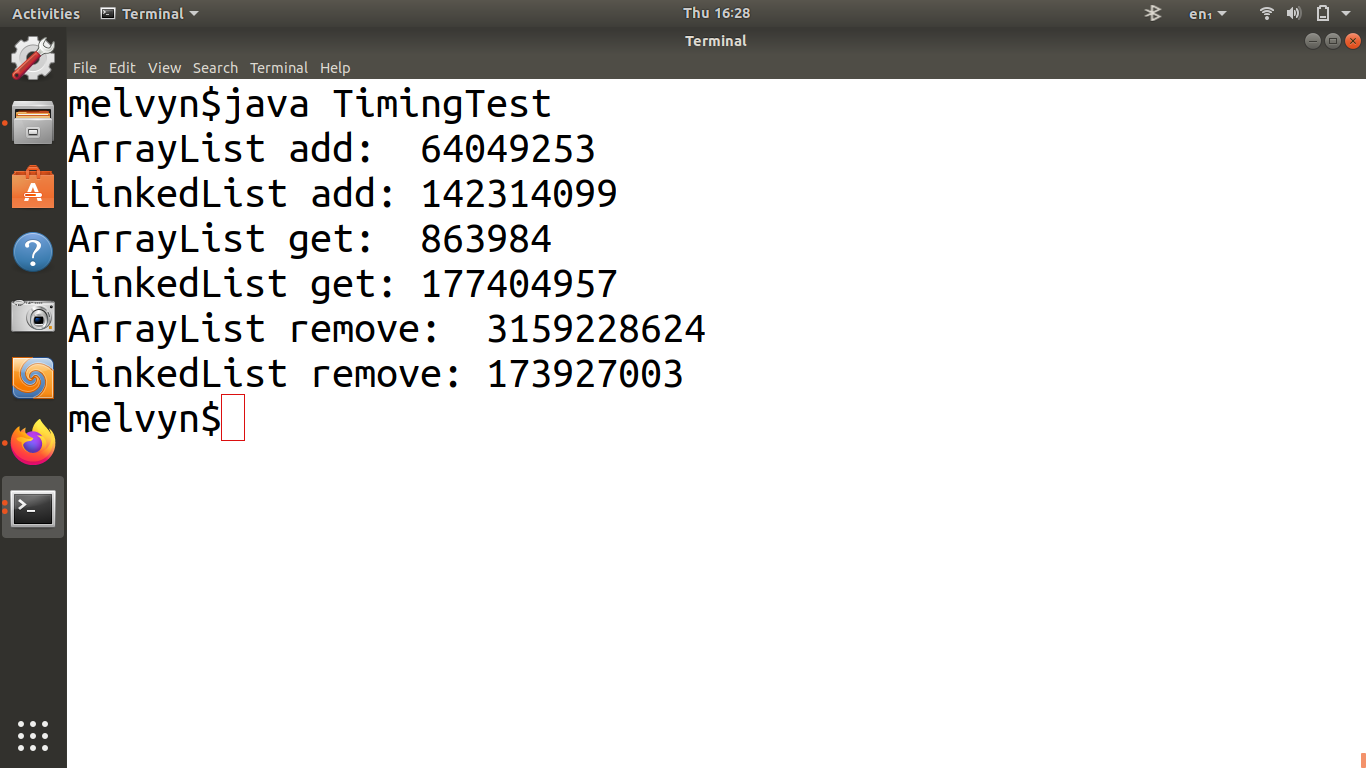
\includegraphics[width=\textwidth]{outputOfTimingTest.png}
  \caption{Comparison of some operators}
\end{figure}


\subsection{ArrayList vs LinkedList dramatic runtime diffference and memory
usage}

Run this code in front of the class. Compare the run times.

Look at this link
\url{https://stackoverflow.com/questions/42849486/why-does-linked-list-delete-and-insert-operation-have-complexity-of-o1-shoul/42849562}

Here's the code:

\lstinputlisting[style=java]{MiddleInsertionComparison.java}


You will see that 

The lets look at the output of the code.

\begin{figure}[h]
  \centering
    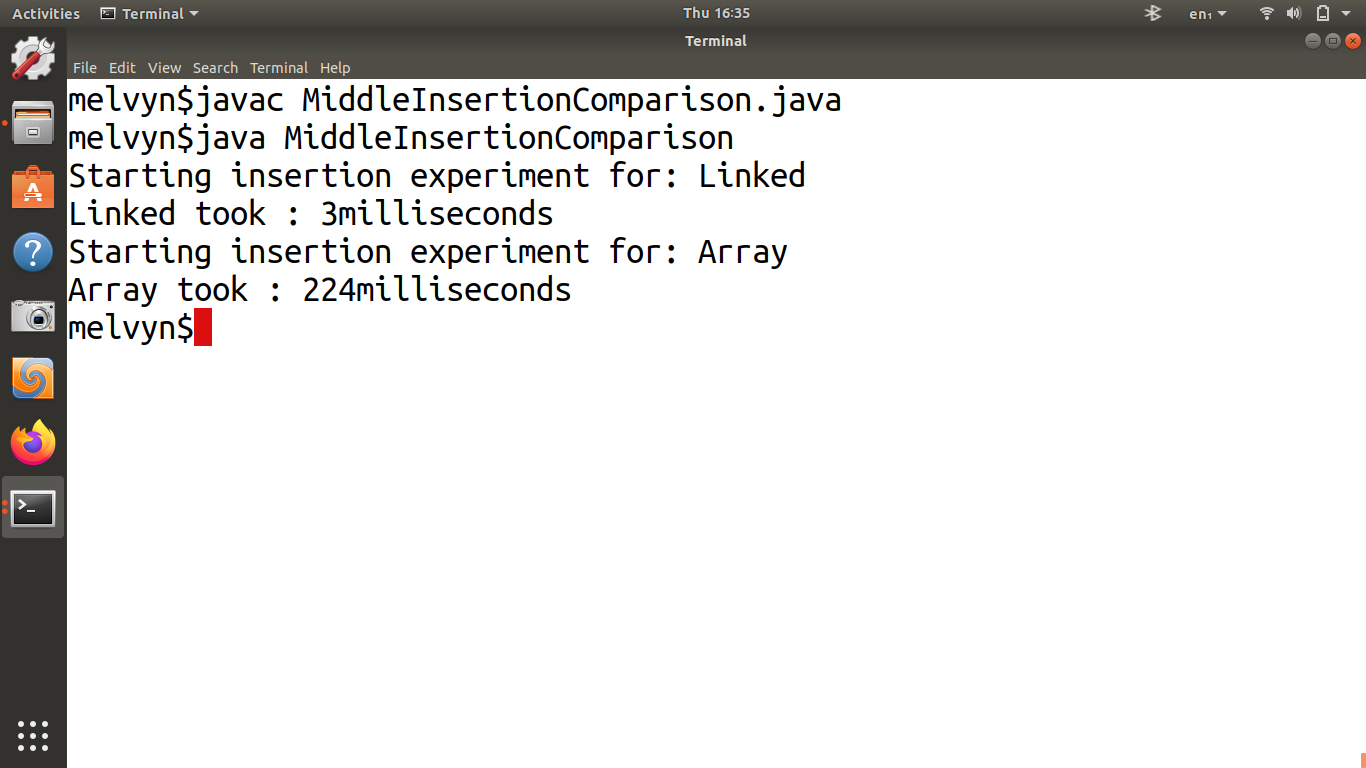
\includegraphics[width=\textwidth]{middleInsertionComparison.png}
  \caption{Compare ArrayList vs LinkedList middle insertion}
\end{figure}


\section{Why Are Collections Useful?}
In case I haven't made it abundantly clear through examples by now, collections are very useful and interesting. Here is the official pitch from Oracle about why Java collections are useful:
\url{file:///home/melvyn/Desktop/JavaFall2019ClassRepo/ReadingMaterials/tutorial/collections/intro/index.html}

\subsection{highlight these points}
\begin{itemize}
\item reduces effort - you never need to code up a dynamically resizing array, because Java has one, for example
\item increases quality - for example, the linked list implementation you are likely to write will be buggy and slow. The one in the collections framework has been tweaked and perfected by experts for a long time.
\item Interoperability between different APIS - since we all agree to use standard collections, all our code can interact. If everyone used a different linked list implementation you couldn't pass data between different peoples' codes.
\end{itemize}

BTW If you don't know what an \textbf{API} is, it means \textbf{Application Programming Interface}. It pretty much means the publicly facing part of your code that other people can access. That may not be helpful - an example is warranted here.

There is a good chance that you know next to nothing about linked lists outside of what I've told you today. Even if you have studied algorithms and data structures, you probably implemented a very simplistic linked list. Nevertheless, today you learned how to add, and remove elements from a linked list. That is because it has a good API. You, the \textbf{Application Programmer}, only have to know a few functions, you don't need to understand the guts of the whole linked list code to use it. The API is the set of publicly accessible functions that application programmers will use.

\subsection{Quiz: Can you name 5 methods in the Java Collections API?}
What are they?

\end{document}
